% defer/rcuintro.tex

\subsection{Introduction to RCU}
\label{sec:defer:Introduction to RCU}

Suppose that you are writing a parallel real-time program that needs
to access
data that is subject to gradual change, perhaps due to changes in
temperature, humidity, and barometric pressure.
The real-time response constraints on this program are so severe that
it is not permissible to spin or block, thus ruling out locking,
nor is it permissible to use a retry loop, thus ruling out sequence locks.
Fortunately, the temperature and pressure are normally controlled,
so that a default hard-coded set of data is usually sufficient.

However, the temperature, humidity, and pressure occasionally deviate too far
from the defaults, and in such situations it is necessary to provide
data that replaces the defaults.
Because the temperature, humidity, and pressure change gradually,
providing the updated values is not a matter of urgency, though
it must happen within a few minutes.
The program is to use a global pointer imaginatively named \co{gptr}
that is normally \co{NULL}, which indicates that the default values
are to be used.
Otherwise, \co{gptr} points to a structure providing values imaginatively
named \co{a}, \co{b}, and \co{c} that are to be
used in the real-time calculations.

How can we safely provide updated values when needed without impeding
real-time readers?

\begin{figure}[tb]
\begin{center}
\resizebox{3in}{!}{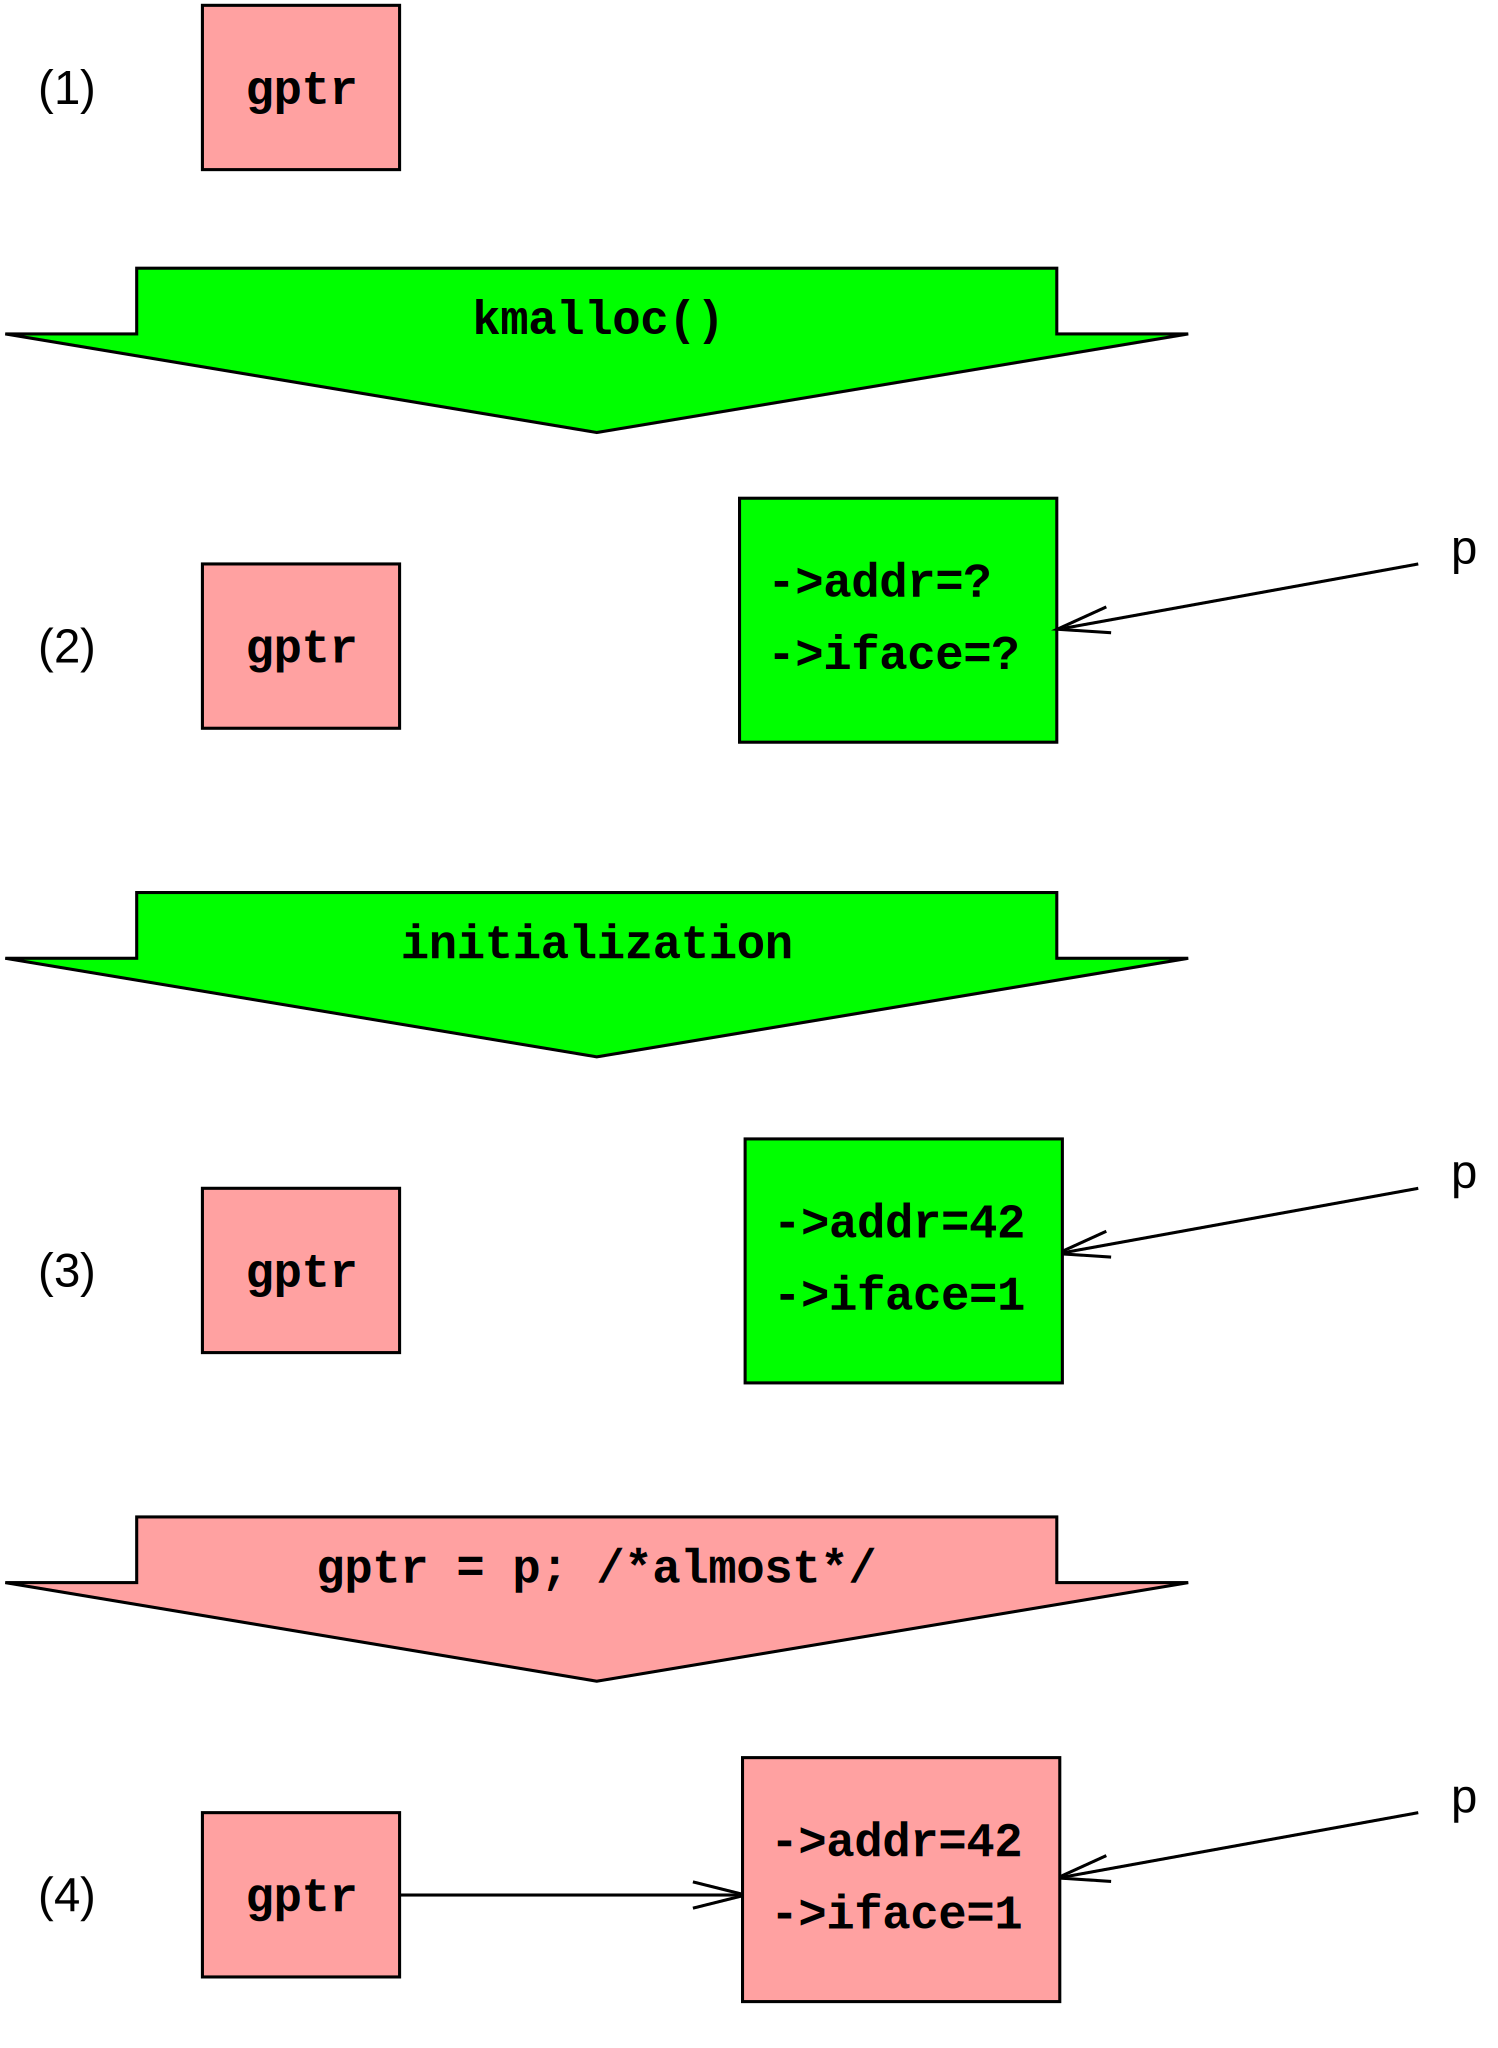
\includegraphics{defer/RCUListInsertClassic}}
\end{center}
\caption{Insertion With Concurrent Readers}
\label{fig:defer:Insertion With Concurrent Readers}
\end{figure}

A classic approach is shown in
Figure~\ref{fig:defer:Insertion With Concurrent Readers}.
The first row shows the default state, with \co{gptr} equal to \co{NULL}.
In the second row, we have allocated a structure which is uninitialized,
as indicated by the question marks.
In the third row, we have initialized the structure.
Next, we assign \co{gptr} to reference this new element.\footnote{
	On many computer systems, simple assignment is insufficient
	due to interference from both the compiler and the CPU.
	These issues will be covered in
	Section~\ref{sec:defer:RCU Fundamentals}.}
On modern general-purpose systems, this assignment is atomic in the
sense that concurrent readers will see either a \co{NULL} pointer
or a pointer to the new structure \co{p}, but not some mash-up
containing bits from both values.
Each reader is therefore guaranteed to either get the
default value of \co{NULL} or to get the newly installed
non-default values, but either way each reader will see
a consistent result.
Even better, readers need not use any expensive synchronization
primitives, so this approach is quite suitable for real-time use.\footnote{
	Again, on many computer systems, additional work is required
	to prevent interference from the compiler, and, on DEC Alpha
	systems, the CPU as well.
	This will be covered in
	Section~\ref{sec:defer:RCU Fundamentals}.}

\begin{figure}[tb]
\begin{center}
\resizebox{3in}{!}{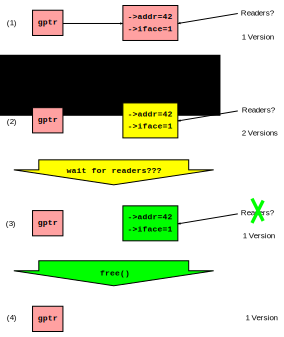
\includegraphics{defer/RCUListDeleteClassic}}
\end{center}
\caption{Deletion From Linked List With Concurrent Readers}
\label{fig:defer:Deletion From Linked List With Concurrent Readers}
\end{figure}

But sooner or later, it will be necessary to remove data that is
being referenced by concurrent readers.
Let us move to a more complex example where we are removing an element
from a linked list, as shown in
Figure~\ref{fig:defer:Deletion From Linked List With Concurrent Readers}.
This list initially contains elements~\co{A}, \co{B}, and \co{C},
and we need to remove element~\co{B}.
First, we use \co{list_del()} to carry out the removal,\footnote{
	And yet again, this approximates reality, which will be expanded
	on in Section~\ref{sec:defer:RCU Fundamentals}.}
at which point all new readers will see element~\co{B} as having been
deleted from the list.
However, there might be old readers still referencing this element.
Once all these old readers have finished, we can safely free
element~\co{B}, resulting in the situation shown at the bottom of
the figure.

But how can we tell when the readers are finished?

It is tempting to consider a reference-counting scheme, but
Figure~\ref{fig:count:Atomic Increment Scalability on Nehalem}
in
Chapter~\ref{chp:Counting}
shows that this can also result in long delays, just as can
the locking and sequence-locking approaches that we already rejected.

Let's consider the logical extreme where the readers do absolutely
nothing to announce their presence.
This approach clearly allows optimal performance for readers
(after all, free is a very good price),
but leaves open the question of how the updater can possibly
determine when all the old readers are done.
We clearly need some additional constraints if we are to provide
a reasonable answer to this question.

One constraint that fits well with some types of real-time operating
systems (as well as some operating-system kernels) is to consider
the case where threads are not subject to preemption.
In such non-preemptible environments, each thread runs until it
explicitly and voluntarily blocks.
This means that an infinite loop without blocking will render a CPU
useless for any other purpose from the start of the infinite loop
onwards.\footnote{
	In contrast, an infinite loop in a preemptible environment
	might be preempted.
	This infinite loop might still waste considerable CPU time,
	but the CPU in question would nevertheless be able to do
	other work.}
Non-preemptibility also requires that threads be prohibited from blocking
while holding spinlocks.
Without this prohibition, all CPUs might be consumed by threads
spinning attempting to acquire a spinlock held by a blocked thread.
The spinning threads will not relinquish their CPUs until they acquire
the lock, but the thread holding the lock cannot possibly release it
until one of the spinning threads relinquishes a CPU.
This is a classic deadlock situation.

Let us impose this same constraint on reader threads traversing the
linked list: such threads are not allowed to block until after
completing their traversal.
Returning to the second row of
Figure~\ref{fig:defer:Deletion From Linked List With Concurrent Readers},
where the updater has just completed executing \co{list_del()},
imagine that CPU~0 executes a context switch.
Because readers are not permitted to block while traversing the linked
list, we are guaranteed that all prior readers that might have been running on
CPU~0 will have completed.
Extending this line of reasoning to the other CPUs, once each CPU has
been observed executing a context switch, we are guaranteed that all
prior readers have completed, and that there are no longer any reader
threads referencing element~\co{B}.
The updater can then safely free element~\co{B}, resulting in the
state shown at the bottom of
Figure~\ref{fig:defer:Deletion From Linked List With Concurrent Readers}.

\begin{figure}[tb]
\begin{center}
\resizebox{3in}{!}{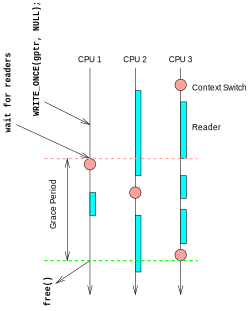
\includegraphics{defer/QSBRGracePeriod}}
\end{center}
\caption{Waiting for Pre-Existing Readers}
\label{fig:defer:Waiting for Pre-Existing Readers}
\end{figure}

A schematic of this approach is shown in
Figure~\ref{fig:defer:Waiting for Pre-Existing Readers},
with time advancing from the top of the figure to the bottom.

Although production-quality implementations of this approach can be
quite complex, a toy implementatoin is exceedingly simple:

\vspace{5pt}
\begin{minipage}[t]{\columnwidth}
\scriptsize
\begin{verbatim}
  1 for_each_online_cpu(cpu)
  2   run_on(cpu);
\end{verbatim}
\end{minipage}
\vspace{5pt}

The \co{for_each_online_cpu()} primitive iterates over all CPUs, and
the \co{run_on()} function causes the current thread to execute on the
specified CPU, which forces the destination CPU to execute a context
switch.
Therefore, once the \co{for_each_online_cpu()} has completed, each CPU
has executed a context switch, which in turn guarantees that
all pre-existing reader threads have completed.

Please note that this approach is \emph{not} production quality.
Correct handling of a number of corner cases and the need for a number
of powerful optimizations mean that production-quality implementations
have significant additional complexity.
In addition, RCU implementations for preemptible environments
require that readers actually do something.
However, this simple non-preemptible approach is conceptually complete,
and forms a good initial basis for understanding the RCU fundamentals
covered in the following section.
